\section{CTST - Lớp 11 - Ôn tập giữa học kì 1 - Đề 1}

\caulc

\Opensolutionfile{ans}[ans-ABCD]

\begin{ex}%[1D1N1-2]%[CTST - Lớp 11 - Ôn tập giữa học kì 1 - Đề 1]%[Tex hóa: Lê Thị Thúy Hằng]
Đổi số đo của góc $\alpha = 120^\circ$ sang đơn vị radian ta được
\choice
{\True $\alpha = \dfrac{2\pi}{3}$}
{$\alpha = \dfrac{\pi}{6}$}
{$\alpha = \dfrac{\pi}{3}$}
{$\alpha = \dfrac{\pi}{4}$}
\loigiai{
	Áp dụng công thức đổi từ độ sang radian ta có: $\alpha^\circ = \alpha \cdot \dfrac{\pi}{180}$ ta có \\
	$$\alpha = 120^\circ = 120 \cdot \dfrac{\pi}{180} = \dfrac{2\pi}{3}.$$
	}
\end{ex}

\begin{ex}%[1D1N2-2]%[CTST - Lớp 11 - Ôn tập giữa học kì 1 - Đề 1]%[Tex hóa: Lê Thị Thúy Hằng]
Cho $\cos \alpha = \dfrac{2}{5}$ với $\dfrac{3\pi}{2} < \alpha < 2\pi$. Tìm giá trị lượng giác của $\sin \alpha$.
\choice
{$\dfrac{21}{25}$}
{$\dfrac{\sqrt{21}}{5}$}
{\True $-\dfrac{\sqrt{21}}{5}$}
{$-\dfrac{21}{25}$}
\loigiai{
	Vì $\dfrac{3\pi}{2} < \alpha < 2\pi$ nên $\sin \alpha < 0$.\\
	Ta có $\sin^2 \alpha + \cos^2 \alpha =1$ nên $\sin \alpha = - \sqrt{1-\cos^2 \alpha}=-\dfrac{\sqrt{21}}{5}$.
}
\end{ex}

\begin{ex}%[1D1N3-1]%[CTST - Lớp 11 - Ôn tập giữa học kì 1 - Đề 1]%[Tex hóa: Lê Thị Thúy Hằng]
Trong các đẳng thức sau, đẳng thức nào \textbf{sai}?
\choice
{$\cos 2\alpha = 1 - 2 \sin^2 \alpha$}
{\True $\tan 2\alpha = \dfrac{2 \tan \alpha}{1+ \tan^2 \alpha}$}
{$\sin 2\alpha = 2 \sin^ \alpha \cos \alpha$}
{$\cos 2\alpha = \cos^2 \alpha - \sin^2 \alpha$}
\loigiai{
	Ta có $\tan 2\alpha = \dfrac{2 \tan \alpha}{1- \tan^2 \alpha}$.
}
\end{ex}

\begin{ex}%[1D1N4-1]%[CTST - Lớp 11 - Ôn tập giữa học kì 1 - Đề 1]%[Tex hóa: Lê Thị Thúy Hằng]
Tập xác định của hàm số $y= \cot x$ là
\choice
{$\mathscr{D}= \mathbb{R} \setminus \left\{ \dfrac{\pi}{2} + k\pi | k \in \mathbb{Z} \right\}$}
{$\mathscr{D}= \mathbb{R} \setminus \left\{ \dfrac{\pi}{4} + k\pi | k \in \mathbb{Z} \right\}$}
{$\mathscr{D}= \mathbb{R} \setminus \left\{ \dfrac{\pi}{8} + k \dfrac{\pi}{2} | k \in \mathbb{Z} \right\}$}
{\True $\mathscr{D}= \mathbb{R} \setminus \left\{k\pi | k \in \mathbb{Z} \right\}$}
\loigiai{
Hàm số $y= \cot x = \dfrac{\sin x}{\cos x}$ xác định khi và chỉ khi \\
$$\sin x \ne 0 \Leftrightarrow x \ne k \pi, k \in \mathbb{Z}.$$
Vậy $\mathscr{D}= \mathbb{R} \setminus \left\{k\pi | k \in \mathbb{Z} \right\}$.
}
\end{ex}

\begin{ex}%[1D1H5-5]%[CTST - Lớp 11 - Ôn tập giữa học kì 1 - Đề 1]%[Tex hóa: Lê Thị Thúy Hằng]
Tập nghiệm của phương trình $2 \sin 2x +1=0$ là
\choice
{\True $S=\left\{ -\dfrac{\pi}{12} + k\pi ; \dfrac{7\pi}{12} + k\pi | k \in \mathbb{Z} \right\}$}
{$S=\left\{ -\dfrac{\pi}{6} + k2\pi ; \dfrac{7\pi}{12} + k2\pi | k \in \mathbb{Z} \right\}$}
{$S=\left\{ -\dfrac{\pi}{12} + k2\pi ; \dfrac{7\pi}{12} + k2\pi | k \in \mathbb{Z} \right\}$}
{$S=\left\{ -\dfrac{\pi}{6} + k\pi ; \dfrac{7\pi}{12} + k\pi | k \in \mathbb{Z} \right\}$}
\loigiai{
Ta có
\begin{eqnarray*}
	& & 2 \sin 2x +1=0 \\
	& \Leftrightarrow & \sin 2x = -\dfrac{1}{2} \\
	& \Leftrightarrow & \sin 2x = \sin \left( -\dfrac{\pi}{6} \right) \\
	& \Leftrightarrow & \hoac{&2x=-\dfrac{\pi}{6}+k2\pi\\&2x=\dfrac{7\pi}{6}+k2\pi}, k \in \mathbb{Z} \\
	& \Leftrightarrow & \hoac{&x=-\dfrac{\pi}{12}+k\pi\\&x=\dfrac{7\pi}{12}+k\pi}, k \in \mathbb{Z}.
\end{eqnarray*}
Vậy tập nghiệm của phương trình $2 \sin 2x +1=0$ là $S=\left\{ -\dfrac{\pi}{12} + k\pi ; \dfrac{7\pi}{12} + k\pi | k \in \mathbb{Z} \right\}$.
}
\end{ex}

\begin{ex}%[1D2N1-3]%[CTST - Lớp 11 - Ôn tập giữa học kì 1 - Đề 1]%[Tex hóa: Lê Thị Thúy Hằng]
Cho dãy số $(u_n)$ thỏa mãn $u_n = 2^{n-1}$. Tìm số hạng thứ $10$ của dãy số đã cho.
\choice
{$2^{11}$}
{\True $2^9$}
{$2^{10}$}
{$2^8$}
\loigiai{
Ta có $u_{10} = 2^{10-1}=2^9$.
}
\end{ex}

\begin{ex}%[1D2N2-4]%[CTST - Lớp 11 - Ôn tập giữa học kì 1 - Đề 1]%[Tex hóa: Lê Thị Thúy Hằng]
Cho cấp số cộng $(u_n)$ có số hạng đầy $u_1 =-3$, công sai $d=2$. Tìm số hạng thứ $5$ của cấp số cộng đó.
\choice
{$u_5=-5$}
{$u_5=-1$}
{$u_5=1$}
{\True $u_5=5$}
\loigiai{
Áp dụng công thức số hạng tổng quát của cấp số cộng ta có $u_5 =u_1 +4d = -3 + 4 \cdot 2 =5$.
}
\end{ex}

\begin{ex}%[1D2H2-4]%[CTST - Lớp 11 - Ôn tập giữa học kì 1 - Đề 1]%[Tex hóa: Lê Thị Thúy Hằng]
	Cho cấp số nhân $(u_n)$ có $u_3=18$; $u_5=162$. Số $1458$ là số hạng thứ bao nhiêu của cấp số nhân đó, biết rằng cấp số nhân có công bội dương.
\choice
{\True Số hạng thứ bảy}
{Số hạng thứ sáu}
{Số hạng thứ tám}
{Số hạng thứ chín}
\loigiai{
	Áp dụng công thức của số hạng tổng quát $u_n = u_1 q^{n-1}$. Ta có:\\
	$\heva{&u_3=u_1 q^2\\&u_5=u_1 q^4} \Rightarrow u_5=u_3 q^2 \Rightarrow 162=18 q^2 \Rightarrow q=3$.\\
	Khi đó $u_1=2$. Vậy $u_n =2 \cdot 3^{n-1}$. \\
	Giả sử 
	$u_n=1458 \Rightarrow 2 \cdot 3^{n-1} =1458 \Rightarrow n=7$.\\
	Vậy $1458$ là số hạng thứ bảy của cấp số nhân.
}
\end{ex}

\begin{ex}%[1H4H1-3]%[CTST - Lớp 11 - Ôn tập giữa học kì 1 - Đề 1]%[Tex hóa: Lê Thị Thúy Hằng]
	Cho tứ diện $ABCD$. Gọi $G$ là trọng tâm của tam giác $BCD$. Giao tuyến của mặt phẳng $(ACD)$ và $(GAB)$ là
\choice
{$AM$ ($M$ là trung điểm của $AB$)}
{\True $AN$ ($N$ là trung điểm của $CD$)}
{$AH$ ($H$ là hình chiếu của $B$ trên $CD$)}
{$AK$ ($K$ là hình chiếu của $C$ trên $BD$)}
\loigiai{
	\immini{
	$A$ là điểm chung thứ nhất của hai mặt phẳng $(ACD)$ và $(GAB)$.\\
	Trong mặt phẳng $(BCD)$, $BG$ cắt $CD$ tại $N$ nên
	$\heva{&N \in BG \subset (ABG)\\&N \in CD \subset (ACD)} \Rightarrow \heva{&N \in (ABG)\\&N \in (ACD)}$. \\
	Suy ra $N$ là điểm chung thứ hai của hai mặt phẳng $(ACD)$ và $(GAB)$.\\
	Vậy $(GAB) \cap (ACD) =AN$.
	}
{
	\begin{tikzpicture}[scale=0.8, font=\footnotesize, line join=round, line cap=round, >=stealth, line join=round]
		\path
		(0:0) coordinate (B)
		++ (0:4) coordinate (D)
		++ (-150:3) coordinate (C)
		(B)++(80:4) coordinate (A)
		($(C)!0.5!(D)$) coordinate (N)
		($(B)!2/3!(N)$) coordinate (G)
		;
		\draw[dashed]
		(N)--(B)--(D)
		(A)--(G)
		;
		\draw
		(A)--(B)--(C)--(D)--(A)--(C)
		;
		\foreach \x/\g in {A/90,B/180,C/-90,D/0,N/-30,G/-90}
			\draw[fill=black] (\x) circle (0.02)+ (\g:.3)
			node{$\x$}
		;
	\end{tikzpicture}
}	
}
\end{ex}

\begin{ex}%[1H4N2-3]%[CTST - Lớp 11 - Ôn tập giữa học kì 1 - Đề 1]%[Tex hóa: Lê Thị Thúy Hằng]
	Cho hình chóp $S.ABCD$ có đáy $ABCD$ là hình thang $(AB \parallel CD)$. Giao tuyến của hai mặt phẳng $(SAB)$ và $(SCD)$ là đường nào?
\choice
{\True Đường thẳng qua $S$ và song song với $AB$ và $CD$}
{Đường thẳng qua $S$ và song song với $AD$ và $BC$}
{Đường thẳng qua $S$ và giao điểm của $AD$ và $BC$}
{Đường thẳng qua $S$ và giao điểm của $AC$ và $BD$}
\loigiai{
\immini{
	$A$ là điểm chung thứ nhất của hai mặt phẳng $(ACD)$ và $(GAB)$.\\
	Trong mặt phẳng $(BCD)$, $BG$ cắt $CD$ tại $N$ nên
	$\heva{&N \in BG \subset (ABG)\\&N \in CD \subset (ACD)} \Rightarrow \heva{&N \in (ABG)\\&N \in (ACD)}$. \\
	Suy ra $N$ là điểm chung thứ hai của hai mặt phẳng $(ACD)$ và $(GAB)$.\\
	Vậy $(GAB) \cap (ACD) =AN$.
}
{
	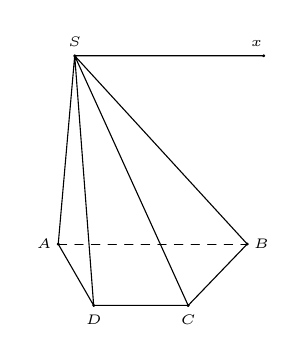
\begin{tikzpicture}[scale=0.6, font=\tiny, line join=round, line cap=round, >=stealth, line join=round]
		\path
		(0:0) coordinate (B)
		++ (180:4) coordinate (A)
		++ (-60:1.5) coordinate (D)
		++ (0:2) coordinate (C)
		(A)++(85:4) coordinate (S)
		++ (0:4) coordinate (x)
		;
		\draw[dashed]
		(A)--(B)
		;
		\draw
		(S)--(A)--(D)--(C)--(B)--cycle
		(D)--(S)--(C)
		(S)--(x)
		;
		\foreach \x/\g in {A/180,B/0,C/-90,D/-90,S/90,x/120}
		\draw[fill=black] (\x) circle (0.02)+ (\g:.3)
		node{$\x$}
		;
	\end{tikzpicture}
}	
}
\end{ex}

\begin{ex}%[1H4H3-2]%[CTST - Lớp 11 - Ôn tập giữa học kì 1 - Đề 1]%[Tex hóa: Lê Thị Thúy Hằng]
	Cho tứ diện $ABCD$ có $M$, $N$ lần lượt là trung điểm của $AB$, $AC$. Mặt phẳng nào sau đây song song với đường thẳng $MN$?
\choice
{$(ACD)$}
{$(ABD)$}
{$(ABC)$}
{\True $(BCD)$}
\loigiai{
	\immini{
		Vì $M$, $N$ lần lượt là trung điểm của $AB$, $AC$ nên $MN$ là đường trung bình của tam giác $ABC$. Do đó, $MN \parallel BC$.\\
		Mà $MN \nsubseteq (BCD)$ và $BC \subset (BCD)$ nên $MN \parallel (BCD)$.
	}
	{
		\begin{tikzpicture}[scale=0.6, font=\footnotesize, line join=round, line cap=round, >=stealth, line join=round]
			\path
			(0:0) coordinate (A)
			++ (0:4) coordinate (C)
			++ (-150:3) coordinate (B)
			(A)++(70:3.5) coordinate (D)
			($(A)!1/2!(B)$) coordinate (M)
			($(A)!1/2!(C)$) coordinate (N)
			;
			\draw[dashed]
			(A)--(C)
			(M)--(N)
			;
			\draw
			(D)--(A)--(B)--(C)--(D)--(B)
			;
			\foreach \x/\g in {A/180,B/-90,C/0,D/90,M/-170,N/70}
			\draw[fill=black] (\x) circle (0.02)+ (\g:.3)
			node{$\x$}
			;
		\end{tikzpicture}
	}
}
\end{ex}

\begin{ex}%[1H4H4-1]%[CTST - Lớp 11 - Ôn tập giữa học kì 1 - Đề 1]%[Tex hóa: Lê Thị Thúy Hằng]
	Cho hai mặt phẳng song song $(\alpha)$ và $(\beta)$, $a$ là đường thẳng bất kì. Tìm mệnh đề \textbf{sai}.
\choice
{Nếu $a$ cắt mp$(\alpha)$ thì $a$ cắt mp$(\beta)$}
{Nếu $a \subset (\alpha)$ thì $a$ song song với mp $(\beta)$}
{Nếu $a \subset (\beta)$ thì $a$ song song với mp $(\alpha)$}
{\True Nếu $a$ song song với mp$(\alpha)$ thì $a$ song song với mp$(\beta)$}
\loigiai{
	Nếu $a$ song song với mp$(\alpha)$ thì $a$ song song với mp$(\beta)$
}
\end{ex}
\Closesolutionfile{ans}

\indapan{6}{ans-ABCD}

\cauds

\Opensolutionfile{ans}[ans-DS]

\begin{ex}%[1D1V3-5]%[CTST - Lớp 11 - Ôn tập giữa học kì 1 - Đề 1]%[Tex hóa: Lê Thị Thúy Hằng]
	Cho góc lượng giác $\alpha = \dfrac{25\pi}{6}$ và $\sin x = -\dfrac{5}{8}$ với $x \in \left(-\dfrac{\pi}{2};0 \right)$.
\choiceTF
{\True $\alpha = \dfrac{25\pi}{6} = 750^\circ$}
{Điểm biểu diễn trên đường tròn lượng giác của góc $\alpha$ thuộc góc phần tư thứ IV}
{$\cos (x + \alpha)=\dfrac{3 \sqrt{13}-5}{16}$}
{\True $P= \dfrac{\sqrt{6}\tan x}{-5\tan^2 x-4}=\dfrac{15\sqrt{26}}{281}$}
\loigiai
{
% Lời giải chung
\begin{itemchoice}
\itemch Đúng. \\
Ta có $\alpha = \dfrac{25\pi}{6} = \left( \dfrac{25\pi}{6} \cdot \dfrac{180}{\pi} \right)^\circ=750^\circ$.
\itemch Sai. \\
Ta có $\alpha = \dfrac{25\pi}{6} = \dfrac{\pi}{6} +4\pi$. Do đó, điểm biểu diễn trên đường tròn lượng giác của góc $\alpha$ thuộc góc phần tư thứ I.
\itemch Sai. \\
Vì $x \in \left(-\dfrac{\pi}{2};0 \right)$ nên $\cos x >0$. Do đó, $\cos x = \sqrt{1-\sin^2 x} =\sqrt{1-\left(-\dfrac{5}{8} \right)^2} =\dfrac{\sqrt{39}}{8}$. \\
Ta có $\sin \alpha = \sin \dfrac{25\pi}{6} = \sin \left( \dfrac{\pi}{6} +4\pi \right) = \sin \dfrac{\pi}{6} = \dfrac{1}{2}$,\\
$\cos \alpha = \cos \dfrac{25\pi}{6} = \cos \left( \dfrac{\pi}{6} +4\pi \right) = \cos \dfrac{\pi}{6} = \dfrac{\sqrt{3}}{2}$.\\
Khi đó, 
\begin{eqnarray*}
	\cos (x + \alpha) 
	& = & \cos x \cos \alpha - \sin x \sin \alpha \\
	& = & \dfrac{\sqrt{39}}{8} \cdot \dfrac{\sqrt{3}}{2} - \left( -\dfrac{5}{8} \right) \cdot \dfrac{1}{2} \\
	& = & \dfrac{3 \sqrt{13}+5}{16}.
\end{eqnarray*}
\itemch Đúng. \\
Ta có $\tan x = \dfrac{\sin x}{\cos x} = \dfrac{-\tfrac{5}{8}}{\tfrac{\sqrt{39}}{8}} = -\dfrac{5\sqrt{39}}{39}$.\\
Khi đó, $P= \dfrac{\sqrt{6}\tan x}{-5\tan^2 x-4}=
=\dfrac{\sqrt{6} \left( -\tfrac{5\sqrt{39}}{39}\right)}{-5 \left( -\tfrac{5\sqrt{39}}{39}\right)^2 -4} =
\dfrac{15\sqrt{26}}{281}$.
\end{itemchoice}
}
\end{ex}

\begin{ex}%[1D1V5-5]%[CTST - Lớp 11 - Ôn tập giữa học kì 1 - Đề 1]%[Tex hóa: Lê Thị Thúy Hằng]
	Cho hàm số $y=f(x)=\sqrt{3} \tan \left(2x-\dfrac{\pi}{3} \right)$.
	\choiceTF
	{Tập xác định của hàm số $\mathscr{D}=\mathbb{R}$}
	{\True Phương trình $f(x)=3$ có nghiệm $x=\dfrac{\pi}{3} + \dfrac{k\pi}{2}$ với $k \in \mathbb{Z}$}
	{Phương trình $f(x)=3$ có nghiệm âm lớn nhất bằng $-\dfrac{\pi}{3}$}
	{\True Khi $-\dfrac{\pi}{4} <x< \dfrac{2\pi}{3}$ thì phương trình $f(x)=3$ có hai nghiệm}
	\loigiai
	{
		% Lời giải chung
		\begin{itemchoice}
			\itemch Sai. \\
			Điều kiện
			$\cos \left(2x-\dfrac{\pi}{3} \right) \ne 0 \Leftrightarrow 2x-\dfrac{\pi}{3} \ne \dfrac{\pi}{2} + k\pi \Leftrightarrow x \ne \dfrac{5\pi}{12} + k\dfrac{\pi}{2}$, $k \in \mathbb{Z}$.
			\itemch Đúng. \\
			Phương trình tương đương với $\tan \left(2x-\dfrac{\pi}{3} \right) = \sqrt{3} \Leftrightarrow x=\dfrac{\pi}{3} + \dfrac{k\pi}{2}$, $k \in \mathbb{Z}$.
			\itemch Sai.\\
			$x <0 \Leftrightarrow \dfrac{\pi}{3} + \dfrac{k\pi}{2} <0 \Leftrightarrow k<-\dfrac{2}{3}$. \\
			Vậy nghiệm âm lớn nhất là $x=\dfrac{\pi}{3}-\dfrac{\pi}{2}=-\dfrac{\pi}{6}$.
			\itemch Đúng. \\
			Có  $-\dfrac{\pi}{4} <x< \dfrac{2\pi}{3} 
			\Leftrightarrow -\dfrac{\pi}{4} < \dfrac{\pi}{3} + \dfrac{k\pi}{2} < \dfrac{2\pi}{3}
			\Leftrightarrow -\dfrac{7}{6} <k< \dfrac{2}{3}$.\\
			Do $k \in \mathbb{Z}$ nên $k \in \left\{-1; 0 \right\}$.\\
			Với $k=-1$ thì $x=-\dfrac{\pi}{6}$.\\
			Với $k=0$ thì $x=\dfrac{\pi}{3}$.\\
			Vậy $x=-\dfrac{\pi}{6}$, $x=\dfrac{\pi}{3}$ thỏa mãn yêu cầu bài toán.
		\end{itemchoice}
	}
\end{ex}

\begin{ex}%[1D2V2-6]%[CTST - Lớp 11 - Ôn tập giữa học kì 1 - Đề 1]%[Tex hóa: Lê Thị Thúy Hằng]
Cho dãy số $(u_n)$ biết $\heva{&u_1=-1\\&u_{n+1}=u_n +3}$ với $n \ge 1$.
	\choiceTF
	{Dãy số trên là một cấp số nhân}
	{Số hạng thứ năm của dãy số là $13$}
	{\True $101$ là số hạng thứ $35$ của dãy số đã cho}
	{\True Tổng các số hạng từ số hạng thứ $10$ đến số hạng thứ $20$ của dãy số bằng $451$.}
	\loigiai
	{
		% Lời giải chung
		\begin{itemchoice}
			\itemch Sai. \\
			Ta có $u_{n+1}=u_n +3$ suy ra dãy số $(u_n)$ là cấp số cộng với công sai $d=3$.
			\itemch Sai. \\
			$u_5 = u_1 +4d=-1+ 4 \cdot 3 =11$. 
			\itemch Đúng. \\
			Xét $u_n=101 \Leftrightarrow 3n-4=101 \Leftrightarrow n=35$.\\
			Vậy $101$ là số hạng thứ $35$ của dãy số đã cho.
			\itemch Đúng. \\
			Ta có \\
			$S_9 = \dfrac{9(2u_1+8d)}{2} = \dfrac{9[2\cdot (-1)+8 \cdot 3]}{2} =99$,\\
			$S_{20} = \dfrac{20(2u_1+19d)}{2} = \dfrac{920[2\cdot (-1)+19 \cdot 3]}{2} =550$. \\
			Vậy $u_{10}+u_{11}+ \cdots + u_{20} = S_{20} - S_9 =550-99=451$.
		\end{itemchoice}
	}
\end{ex}

\begin{ex}%[1H4V4-3]%[CTST - Lớp 11 - Ôn tập giữa học kì 1 - Đề 1]%[Tex hóa: Lê Thị Thúy Hằng]
	Cho hình hộp $ABCD.A'B'C'D'$. Gọi $G_1$, $G_2$ lần lượt là trọng tâm của tam giác $A'BD$, $B'D'C$.
	\choiceTF
	{Đường thẳng $A'B$ cắt đường thẳng $CD$.}
	{\True $A'D'CB$ là hình bình hành}
	{\True $(A'B'D) \parallel (B'D'C)$}
	{$G_1 G_2 = \dfrac{2}{3}AC$}
	\loigiai
	{
	\begin{center}
		\begin{tikzpicture}[>=stealth,line join=round,line cap=round,font=\footnotesize,scale=1]
			\def\a{3};
			\def\cao{2.5};
			\def\g{-160};
			\path
			(0:0) coordinate (A)
			(0:\a) coordinate (B)
			(\g:{\a/2}) coordinate (D)
			($(B)+(D)-(A)$) coordinate (C)
			($(A)+(-85:\cao)$) coordinate (A')
			($(B)+(-85:\cao)$) coordinate (B')
			($(C)+(-85:\cao)$) coordinate (C')
			($(D)+(-85:\cao)$) coordinate (D')
			;
			\draw
			(A)--(B)--(C)--(D)--cycle 
			(D)--(D')--(C')--(C)--(B')--(B)
			(C')--(B')
			(D')--(C)
			;
			\draw[dashed] 
			(A)--(A')--(D)
			(D')--(A')--(B')--cycle
			(A')--(B)
			;
			\foreach \x/\g in {A/90,B/0,C/90,D/180,A'/180,B'/0,C'/-45,D'/180}\fill[black](\x) circle (1pt) +(\g:3mm) node {$\x$};
			%\foreach \x/\y/\z in {}{\draw pic[draw,angle radius=2mm]{right angle=\x--\y--\z};}
		\end{tikzpicture}
	\end{center}
		% Lời giải chung
		\begin{itemchoice}
			\itemch Sai. \\
			Do $A' \notin (BCD)$ nên đường thẳng $A'B$ và đường thẳng $CD$ chéo nhau.
			\itemch Đúng. \\
			Vì $ABCD.A'B'C'D'$ là hình hộp nên $A'D' \parallel BC$ và $A'D' = BC$. Do đó, $A'D'CB$ là hình bình hành.
			\itemch Đúng. \\
			Vì $A'D'CB$ là hình bình hành nên $A'B \parallel CD'$, suy ra $A'B \parallel (B'D'C)$. \quad (1) \\
			Tương tự, ta có $A'B' \parallel CD$ và $A'B' = CD$ nên $A'B'CD$ là hình bình hành. Suy ra $A'D \parallel B'C$. Do đó,  $A'D \parallel (B'D'C)$. \quad (2) \\
			Từ (1) và (2) suy ra $(A'B'D) \parallel (B'D'C)$.
			\itemch Sai. \\
			\immini{
			Gọi $O$, $O'$, $I$ theo thứ tự là tâm của các hình bình hành $ABCD$, $A'B'C'D'$, $ACC'A'$.\\
			Vì $G_1$ là trọng tâm tam giác $AB'D$ nên $\dfrac{A'G_1}{AO} = \dfrac{2}{3}$, do đó $G_1$ là trọng tâm tam giác $A'AC$. Vậy $G_1 = AI \cap A'O$. \quad (3)\\
			Tương tự, vì $G_2$ là trọng tâm tam giác $B'D'C$ nên $\dfrac{CG_2}{CO} = \dfrac{2}{3}$, do đó $G_2$ là trọng tâm tam giác $A'C'C$. Vậy $G_2 = C'I \cap CO'$. \quad (4) \\
			}{\begin{tikzpicture}[>=stealth,line join=round,line cap=round,font=\footnotesize,scale=0.8]
				\def\a{5};
				\def\cao{3.5};
				\def\g{-120};
				\path
				(0:0) coordinate (A)
				(0:\a) coordinate (B)
				(\g:{\a/2}) coordinate (D)
				($(B)+(D)-(A)$) coordinate (C)
				($(A)+(-85:\cao)$) coordinate (A')
				($(B)+(-85:\cao)$) coordinate (B')
				($(C)+(-85:\cao)$) coordinate (C')
				($(D)+(-85:\cao)$) coordinate (D')
				($(B)!1/2!(D)$) coordinate (O)
				($(B')!1/2!(D')$) coordinate (O')
				($(A')!1/2!(C)$) coordinate (I)
				($(A)!2/3!(I)$) coordinate (G_1)
				($(C')!2/3!(I)$) coordinate (G_2)
				;
				\draw
				(A)--(B)--(C)--(D)--cycle 
				(D)--(D')--(C')--(C)--(B')--(B)--cycle
				(C')--(B')
				(D')--(C)--(A)
				
				;
				\draw[dashed] 
				(A)--(A')--(D)
				(D')--(A')--(B')--cycle
				(A)--(C')--(A')--(B)
				(A')--(C)
				;
				\foreach \x/\g in {A/90,B/0,C/90,D/180,A'/-170,B'/0,C'/-45,D'/180,O/90,O'/90,I/90,G_1/180,G_2/0}\fill[black](\x) circle (1pt) +(\g:3mm) node {$\x$};
				%\foreach \x/\y/\z in {}{\draw pic[draw,angle radius=2mm]{right angle=\x--\y--\z};}
			\end{tikzpicture}
			}
				Từ (3) và (4) suy ra $G_1$, $G_2$ cùng thuộc $AC'$. \\
				Ta có $\dfrac{AG_1}{AI}= \dfrac{2}{3} \Rightarrow \dfrac{AG_1}{AC'}= \dfrac{1}{3}$;
				$\dfrac{C'G_2}{C'I}= \dfrac{2}{3} \Rightarrow \dfrac{C'G_2}{AC'}= \dfrac{1}{3}$.\\
				Do đó, $AG_1 = G_1 G_2 = G_2 C' = \dfrac{1}{3} AC'$.\\
				Vậy $G_1$, $G_2$ cùng thuộc $AC'$, đồng thời chia $AC'$ thành ba phần bằng nhau.
		\end{itemchoice}
	}
\end{ex}
\Closesolutionfile{ans}

\indapan{3}{ans-DS}

\caukq

\Opensolutionfile{ans}[ans-KQ]

\begin{ex}%[1D1V1-5]%[CTST - Lớp 11 - Ôn tập giữa học kì 1 - Đề 1]%[Tex hóa: Lê Thị Thúy Hằng]
	Gọi $M$, $N$, $E$ là các điểm trên đường tròn lượng giác sao cho số đo của các góc lượng giác $(OA,OM)$, $(OA,ON)$, $(OA,OE)$ lần lượt bằng $-\dfrac{\pi}{2}$; $-\dfrac{7\pi}{6}$; $\dfrac{\pi}{6}$. Khi đó, diện tích tam giác $MNE$ làm tròn đến hàng phần chục bằng bao nhiêu? 
\shortans{$1{,}3$}
\loigiai
{
	Trên đường tròn lượng giác đi theo chiều dương từ vị trí điểm gốc $A$, thứ tự các điểm lần lượt là $E$; $N$; $M$ và $\widehat{EON} = \widehat{NOM} = \widehat{MOE} = \dfrac{2\pi}{3}$.\\
	Mà $OE=ON=OM=1$ nên $EN=NM=ME$. Do đó, tam giác $MNE$ là tam giác đều cạnh $MN = \sqrt{3}$. Vậy $S_{MNE} = \dfrac{(\sqrt{3})^2 \cdot \sqrt{3}}{4} = \dfrac{3 \sqrt{3}}{4} \approx 1{,}3$.
}
\end{ex}

\begin{ex}%[1D1C3-5]%[CTST - Lớp 11 - Ôn tập giữa học kì 1 - Đề 1]%[Tex hóa: Lê Thị Thúy Hằng]
	Tính $S= \sin \dfrac{\pi}{2024} + \sin \dfrac{2\pi}{2024} + \sin \dfrac{3\pi}{2024} + \cdots + \sin \dfrac{2023\pi}{2024}$. Kết quả làm tròn đến hàng đơn vị.
	\shortans{$1289$}
	\loigiai
	{
	Xét bài toán tổng quát. Tính tổng
	$S= \sin x + \sin 2x + \cdots + \sin (n-1)x$ \quad (1).\\
	Nhân cả hai vế (1) với $2 \sin \dfrac{x}{2}$ ta có\\
	\begin{eqnarray*}
		 & & 2 \sin \dfrac{x}{2} S = 2 \sin \dfrac{x}{2} \sin x + 2 \sin \dfrac{x}{2} \sin 2x + \cdots + 2 \sin \dfrac{x}{2} \sin (n-1)x\\
		 & \Rightarrow & 2 \sin \dfrac{x}{2} S = \left( \cos \dfrac{x}{2} - \cos \dfrac{3x}{2} \right) + \left( \cos \dfrac{3x}{2} - \cos \dfrac{5x}{2} \right) + \cdots + \left[ \cos \left( \dfrac{2n-3}{2} \right)x - \cos \left( \dfrac{2n-1}{2} \right)x \right] \\
		 & \Rightarrow & 2 \sin \dfrac{x}{2} S = \cos \dfrac{x}{2} - \cos \left( \dfrac{2n-1}{2} \right)x \\
		 & \Rightarrow & 2 \sin \dfrac{x}{2} S = 2 \sin \dfrac{(n-1)x}{2} \sin \dfrac{nx}{2} \\
		 & \Rightarrow & S= \dfrac{\sin \tfrac{(n-1)x}{2} \sin \tfrac{nx}{2}}{\sin \tfrac{x}{2}}.
	\end{eqnarray*}
	Áp dụng với $x= \dfrac{\pi}{2024}$ và $n=2024$ ta được
	$S_2 = \dfrac{\sin \tfrac{2023 \pi}{2 \cdot 2024} \sin \tfrac{\pi}{2}}{\sin \tfrac{\pi}{2 \cdot 2024}} = \dfrac{\sin \tfrac{2023 \pi}{2 \cdot 2024}}{\sin \tfrac{\pi}{2 \cdot 2024}} \approx 1289$.
	}
\end{ex}

\begin{ex}%[1D1V5-6]%[CTST - Lớp 11 - Ôn tập giữa học kì 1 - Đề 1]%[Tex hóa: Lê Thị Thúy Hằng]
	Một chất điển dao động điều hòa theo phương trình $x= 2 \cos \left( 2\pi t + \dfrac{\pi}{2} \right)$, $t$ tính bằng giây và $x$ tính bằng cm. Gọi $t_o$ là thời điểm đầu tiên vật có li độ lớn nhất. Giá trị của $t_o$ bằng bao nhiêu giây?
	\shortans{$0{,}75$}
	\loigiai
	{
	Với mọi $t \ge 0$ ta có $-1 \le \cos \left( 2\pi t + \dfrac{\pi}{2} \right) \le 1 \Leftrightarrow -2 \le 2 \cos \left( 2\pi t + \dfrac{\pi}{2} \right) \le 2$.\\
	Do đó, li độ lớn nhất là $x=2$ cm xảy ra khi \\
	$ \cos \left( 2\pi t + \dfrac{\pi}{2} \right) =1 \Leftrightarrow 2\pi t + \dfrac{\pi}{2} = k2\pi \Leftrightarrow t = k - \dfrac{1}{4}$, $k \in \mathbb{Z}$.\\
	Vì $t \ge 0$ nên $k- \dfrac{1}{4} \ge 0 \Leftrightarrow k \ge \dfrac{1}{4}$.\\
	Vì $k \in \mathbb{Z}$ nên thời điểm đầu tiên thỏa mãn ứng với $k=1 \Rightarrow t_0 = \dfrac{3}{4} = 0{,}75$ giây.
	}
\end{ex}

\begin{ex}%[1D2V2-5]%[CTST - Lớp 11 - Ôn tập giữa học kì 1 - Đề 1]%[Tex hóa: Lê Thị Thúy Hằng]
	Cho dãy số $(u_n)$ xác định bởi $\heva{&u_1=a\\&u_{n+1}=5-u_n, n \ge 1}$. Tìm $a$ để $(u_n)$ là cấp số cộng.
	\shortans{$2{,}5$}
	\loigiai
	{
	Giả sử $(u_n)$ là cấp số cộng. Khi đó, tồn tại một hằng số $d$ sao cho $u_{n+1} -u_n=d \forall n \ge 1$ \quad (1). \\
	Từ hệ thức xác định dãy số $(u_n)$ ta suy ra $u_{n+1} -u_n= 5 - 2 u_n \forall n \ge 1$ \quad (2). \\
	Từ (1) và (2) ta có $u_n = \dfrac{5-d}{2}, \forall n \ge 1$.\\
	$\Rightarrow (u_n)$ là một dãy số không đổi.\\
	$\Rightarrow u_2 =a \Rightarrow a=5-u_1=5-a \Rightarrow a= \dfrac{5}{2}$.\\
	Với $a= \dfrac{5}{2}$, ta cũng chứng minh được $u_n= \dfrac{5}{2}$.\\
	Vậy $a= \dfrac{5}{2}$ là giá trị cần tìm.
	}
\end{ex}

\begin{ex}%[1H4C1-4]%[CTST - Lớp 11 - Ôn tập giữa học kì 1 - Đề 1]%[Tex hóa: Lê Thị Thúy Hằng]
	Cho hình tứ diện đều $ABCD$ có cạnh bằng $12$. Gọi $M$, $N$ lần lượt là trung điểm của cạnh $AB$ và $CD$. Gọi $P$ là trung điểm đoạn thẳng $CM$. Giao điểm $I$ của đường thẳng $DP$ và mặt phẳng $(ABN)$ cách điểm $D$ một khoảng bằng bao nhiêu?
	\shortans{$6{,}63$}
	\loigiai
	{
	\immini{
		Trong mặt phẳng $(DMC)$, gọi $I$ là giao điểm của $MN$ và $DP$.\\
		Khi đó, $I \in MN \subset (ABN) \Rightarrow I \in (ABN)$.\\
		Vậy $I$ là giao điểm của $DP$ và $(ABN)$.\\
		Tam giác $DMC$ có $MN$ và $DP$ là hai đường trung tuyến nên giao điểm $I$ là trọng tâm của tam giác $DMC$.\\
		Ta có tam giác $ABD$ là tam giác đều cạnh bằng $12$ và có $DM$ là đường trung cao nên $DM = 12 \cdot \dfrac{\sqrt{3}}{2} = 6 \sqrt{3}$.\\
		Tương tự ta có $CM = 6 \sqrt{3}$.
	}{\begin{tikzpicture}[>=stealth,line join=round,line cap=round,font=\footnotesize,scale=0.8]
			\def\a{6};
			\def\cao{5.5};
			\def\g{-60};
			\path
			(0:0) coordinate (A)
			(0:\a) coordinate (C)
			(\g:{\a/2}) coordinate (B)
			($(A)+(55:\cao)$) coordinate (D)
			($(A)!1/2!(B)$) coordinate (M)
			($(C)!1/2!(D)$) coordinate (N)
			($(C)!1/2!(M)$) coordinate (P)
			(intersection of D--P and M--N) coordinate (I)
			;
			\draw
			(M)--(D)--(A)--(B)--(D)--(C)--(B)--(N);
			;
			\draw[dashed] 
			(N)--(M)--(C)--(A)--cycle
			(D)--(P)
			;
			\foreach \x/\g in {A/180,B/-90,C/0,D/90,M/-150,N/0,P/-60,I/180}\fill[black](\x) circle (1pt) +(\g:3mm) node {$\x$};
			%\foreach \x/\y/\z in {}{\draw pic[draw,angle radius=2mm]{right angle=\x--\y--\z};}
		\end{tikzpicture}
	}
	\noindent Do đó, tam giác $DMC$ cân tại $M$. Suy ra $MN$ cũng là đường cao của tam giác $DMC$ hay $MN \perp CD$.\\
	Ta có $DM = 6 \sqrt{3}$, $DN = \dfrac{1}{2} DC = 6$ nên $MN = \sqrt{DM^2 - DN^2} = 6 \sqrt{2}$.\\
	Khi đó, $IN = \dfrac{1}{3} MN = 2 \sqrt{2}$.\\
	Tam giác $DNI$ vuông tại $N$ nên $DI = \sqrt{DN^2 + IN^2} = 2 \sqrt{11}$.\\
	Vậy $I$ cách điểm $D$ một khoảng bằng $2 \sqrt{11} \approx 6{,}63$.
	}
\end{ex}

\begin{ex}%[1H4C4-6]%[CTST - Lớp 11 - Ôn tập giữa học kì 1 - Đề 1]%[Tex hóa: Lê Thị Thúy Hằng]
	Cho hình chóp $S.ABCD$ có đáy $ABCD$ là hình bình hành, $O$ là giao điểm của $AC$ và $BD$. Tam giác $SCD$ là tam giác đều cạnh $2$. Mặt phẳng $(P)$ đi qua $O$ và song song với mặt phẳng $(SCD)$. Tính diện tích hình tạo bởi mặt phẳng $(P)$ và các mặt của hình chóp $S.ABCD$.
	\shortans{$1{,}3$}
	\loigiai
	{
	\begin{center}
		\begin{tikzpicture}[>=stealth,line join=round,line cap=round,font=\footnotesize,scale=0.8]
			\def\a{5.5};
			\def\cao{4};
			\def\g{-135};
			\path
			(0:0) coordinate (A)
			(0:\a) coordinate (D)
			(\g:{\a/3}) coordinate (B)
			($(B)+(D)-(A)$) coordinate (C)
			($(A)+(85:\cao)$) coordinate (S)
			($(A)!1/2!(C)$) coordinate (O)
			($(A)!1/2!(D)$) coordinate (M)
			($(B)!1/2!(C)$) coordinate (N)
			($(S)!1/2!(B)$) coordinate (E)
			($(S)!1/2!(A)$) coordinate (F)
			($(S)!1/2!(C)$) coordinate (I)
			($(S)!1/2!(D)$) coordinate (K)
			;
			\fill[magenta!10!white] (E)--(F)--(M)--(N)--cycle;
			\fill[green!10!white] (I)--(C)--(D)--(K)--cycle;
			\draw
			(S)--(B)--(C)--(S)--(D)--(C)
			(E)--(N)
			(I)--(K)
			;
			\draw[dashed] 
			(S)--(A)--(B)
			(C)--(A)--(D)--(B)
			(E)--(F)--(M)--(N)
			;
			\foreach \x/\g in {A/180,B/-90,C/-90,D/0,S/90,O/-90,M/-70,N/-90,E/180,F/20,I/180,K/30}\fill[black](\x) circle (1pt) +(\g:3mm) node {$\x$};
		\end{tikzpicture}
	\end{center}
	Do $(P) \parallel (SCD)$ mà $(ABCD) \cap (SCD) =CD$ nên   $(ABCD) \cap (P) =MN$. Kết hợp với giả thiết đề bài, suy ra $MN$ đi qua $O$ và song song với $CD$.\\
	Tương tự ta có  $(SAD) \cap (P) =MF \parallel SD$, $(SBC) \cap (P) =NE \parallel SC$.\\
	Vậy hình tạo bởi mặt phẳng $(P)$ và các mặt của hình chóp $S.ABCD$ là tứ giác $MNEF$.\\
	Ta có $MN$ đi qua $O$ và song song với $CD$ nên $M$, $N$ lần lượt là trung điểm của $AD$, $BC$. Do đó, $E$, $F$ lần lượt là trung điểm của $SB$, $SA$.\\
	Gọi $I$, $K$ lần lượt là trung điểm $SC$, $SD$. Khi đó, ta có\\
	$IK \parallel EF$, $IK = EF$, $IC \parallel EN$, $IC = EN$, $KD \parallel FM$, $KD = FM$, $MN \parallel CD$, $MN = CD$.\\
	Vậy ta có diện tích hình thang $MNEF$ là \\
	$S_{MNEF} = S_{DCIK} = \dfrac{3}{4} S_{SCD} = \dfrac{3}{4} \cdot \dfrac{\sqrt{3}}{4} \cdot (2)^2 = \dfrac{3 \sqrt{3}}{4} \approx 1{,}3$.
	}
\end{ex}

\Closesolutionfile{ans}

\indapan{6}{ans-KQ}

